\subsection{时齐马氏链与转移概率}

\begin{definition}[时间齐次马氏链]
    称马氏链 $X:\{X_n,n\geq 0\}$ 为时齐的或时间齐次马氏链, 若对 $\forall n\geq 0, i,j\in S$
    \[
    \PP(X_{n+1}=j|X_n=i)=\PP(X_1=j|X_0=i)
    \]
\end{definition}

\begin{definition}
    $X$ 是时齐马氏链, 称
    \[
    p_{ij}:=p_{i,j}=\PP(X_1=j|X_0=i)\qquad i,j\in S
    \]
    为 $X$ 从状态 $i$ 到 $j$ 的(一步)\textbf{转移概率}, 并称矩阵
    \[
    P=\begin{bmatrix}
        p_{11} & p_{12} & p_{13} & \cdots\\
        p_{21} & p_{22} & p_{23} & \cdots\\
        \vdots & \vdots & \vdots & \ddots
    \end{bmatrix}
    \]
    为(一步)转移(概率)矩阵
\end{definition}

若不加说明, 则默认讨论的马氏链都是时齐的

注:
\[
\begin{aligned}
    \PP(x_{n+1}=y)&=\sum_{x\in S}\PP(X_{n+1}=y|X_n=x)\cdot \PP(X_n=x)\\
    &=\sum_{x\in S}p_{xy}\cdot \PP(X_n=x)
\end{aligned}
\]

\begin{theorem}[转移矩阵的刻画]\label{thm:random_matrix}
    转移矩阵是一个随机矩阵, 即
    \begin{enumerate}
        \item $\forall i,j\in S,p_{ij}\geq 0$
        \item $\forall i\in S,\sum_{j\in S}p_{ij}=1$
    \end{enumerate}
    即转移矩阵的每一行 $(p_{ij})_{j\in S}$ 为 $S$ 上的一个概率分布

    注:另一种随机矩阵是指元素为随机变量的矩阵, 和这里讲的没有关系
\end{theorem}

证明:
\[
\sum_{j\in S}\PP(X_1=j|X_0=i)=\PP(X_1\in S|X_0=i)=\PP(\Omega|X_0=i)=1
\]

\begin{definition}[时齐马氏链]\label{def:homo-markov}
    设 $X=\{X_n,n\geq 0\}$ 为一随机过程, 若
    \begin{enumerate}
        \item 初值 $X_0$ 满足分布 $\mu=(\mu_i)_{i\in S}$, 即 $\PP(X_0=i)=\mu_i,i\in S$
        \item 存在一个随机矩阵 $P=(p_{ij})_{i,j\in S}$ 使得 $\forall n\geq 1,i_0,\cdots,i_{n-1},i,j\in S$
        \[
        \PP(X_{n+1}=j|X_0=i_0,\cdots,X_{n-1}=i_{n-1},X_n=i)=p_{ij}
        \]
    \end{enumerate}
    则称 $X$ 具有初始分布 $\mu$ 和转移矩阵 $P$ 的(时齐)马氏链, 记作 $X\sim \text{Markov}(\mu,P)$
\end{definition}

上述定义与$(M_1)$马氏链定义\ref{def:M_1}等价

证明:$(2)\rightarrow (M_1)$
\[
\begin{aligned}
    \PP(X_{n+1}=j|X_n=i)&=\sum_{(i_0,\cdots,i_{n-1})\in S^n}\PP(X_{n+1}=j|X_n=i,X_0=i_0,\cdots,X_{n-1}=i_{n-1})\PP(X_0=i_0,\cdots,X_{n-1}=i_{n-1})\\
    &=\sum_{(i_0,\cdots,i_{n-1})\in S^n}p_{ij}\cdot \PP(X_0=i_0,\cdots,X_{n-1}=i_{n-1})=p_{ij}
\end{aligned}
\]
所以 $\PP(X_{n+1}=j|X_0=i_0,\cdots,X_{n-1}=i_{n-1},X_n=i)=\PP(X_{n+1}=j|X_n=i)$

即然有 $(M_1)$, 为什么还要定义\ref{def:homo-markov}?因为该定义决定了马氏链的有限维分布

\begin{example}[Gambler's Ruin]
    [Durrett\cite{durrett},P1] 
    \begin{figure}[H]
        \centering
        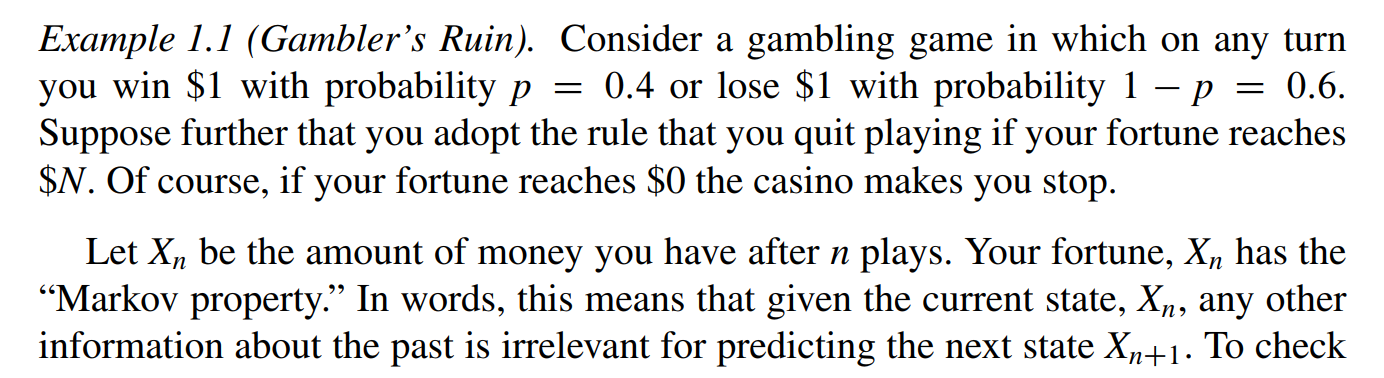
\includegraphics[width=0.9\textwidth]{figures/Gambler's Ruin.png}
        \caption{Gambler's Ruin}
    \end{figure}
\end{example}

\begin{claim}
$\{X_n,n\geq 0\}$ 为(时齐)马氏链
\end{claim}

1. 对于 $0<i_0,\cdots,i_{n-1}<N, n\geq 0$ 有
\[
\begin{aligned}
    &\PP(X_{n+1}=i+1|X_n=i,X_0=i_0,\cdots,X_{n-1}=i_{n-1})\\
    =&\PP(X_{n+1}=i+1|X_n=i)=0.4=\PP(\text{第}n+1\text{次赌局赢一元})
\end{aligned}
\]
\[
\begin{aligned}
    &\PP(X_{n+1}=i-1|X_n=i,X_0=i_0,\cdots,X_{n-1}=i_{n-1})\\
    =&\PP(X_{n+1}=i-1|X_n=i)=0.6=\PP(\text{第}n+1\text{次赌局输一元})
\end{aligned}
\]

2. $\PP(X_{n+1}=0|X_n=0,X_0=i_0,\cdots,X_{n-1}=i_{n-1})=1=\PP(X_{n+1}=0|X_n=0)$

$\PP(X_{n+1}=N|X_n=N, X_0=i_0,\cdots, X_{n-1}=i_{n-1})=1=\PP(X_{n+1}=N|X_n=N)$

最后一个等号是由题目设定得到, 从 $0\to 0$ 或 $N\to N$ 的概率都为1, 因为游戏结束

综上, $p(i,i+1)=0.4,0<i<N, p(i,i-1)=0.6, 0<i<N, p(0,0)=p(N,N)=1$

e.g. 

\begin{figure}[H]
    \centering
    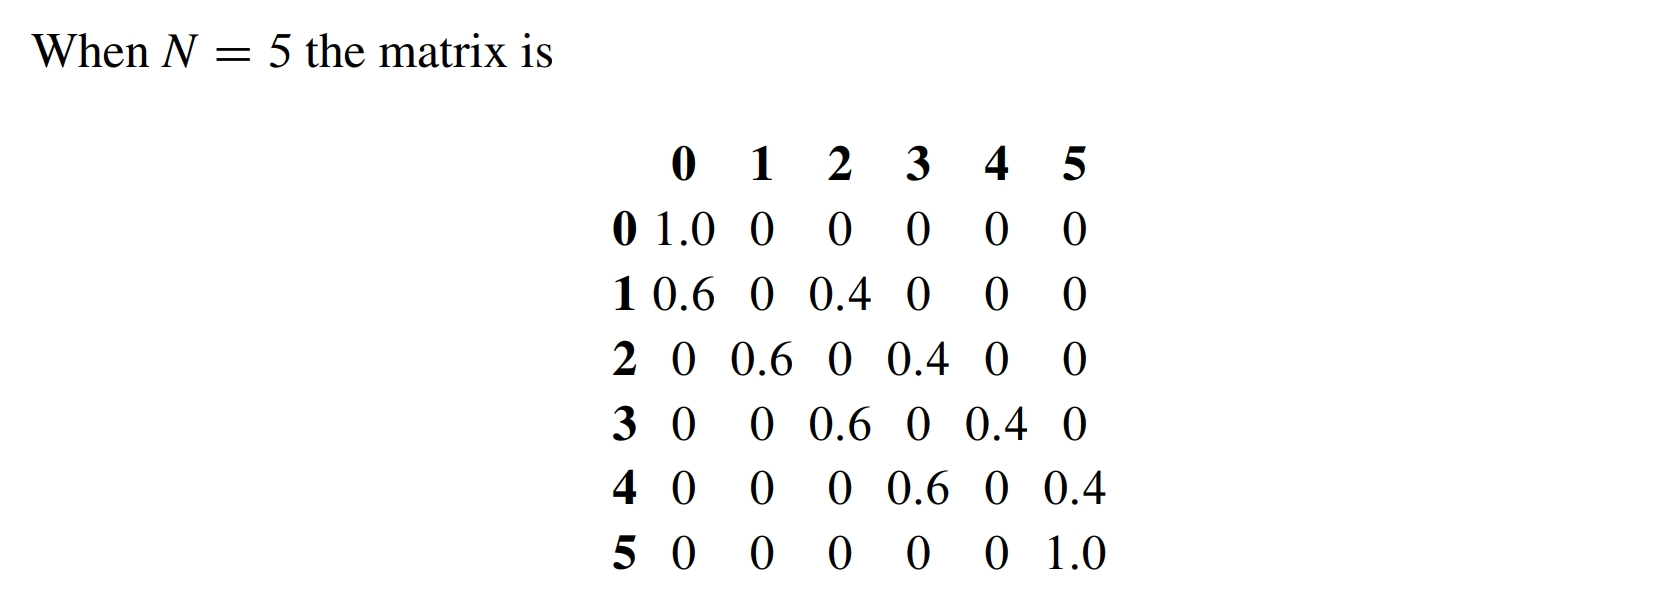
\includegraphics[width=0.9\textwidth]{figures/N=5.png}
    \caption{N=5}
\end{figure}

\begin{example}[Two-Stage Markov Chains]
    [Durrett\cite{durrett}, P7]
    \begin{figure}[H]
        \centering
        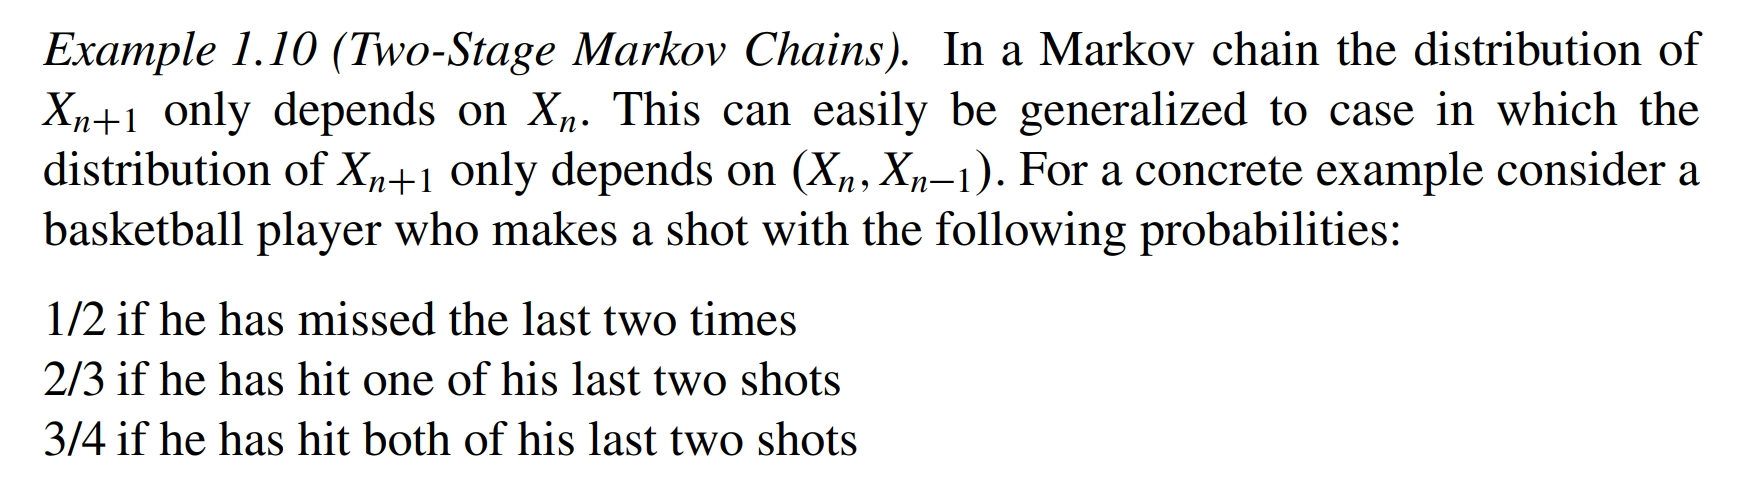
\includegraphics[width=0.9\textwidth]{figures/two_stage_markov_chains.png}
        \caption{Two-Stage Markov Chains}
    \end{figure}
\end{example}

\begin{enumerate}
    \item $\PP(X_{n+1}=H|X_n=M,X_{n-1}=M)=1/2$
    \item $\PP(X_{n+1}=H|X_n=M,X_{n-1}=H)=\PP(X_{n+1}=H|X_n=H,X_{n-1}=M)=2/3$
    \item $\PP(X_{n+1}=H|X_n=H,X_{n-1}=H)=3/4$
\end{enumerate}

\begin{claim}
$Y_n=(X_n,X_{n-1}), n\geq 1$ 则 $\{Y_n,n\geq 1\}$ 是(时齐)马氏链, $Y_n:\Omega\to \{HH,HM,MH,MM\}$ 
\end{claim}

证明:
\[
\begin{aligned}
    &\PP(Y_{n+1}=HH|Y_n=HH,Y_j=(x_j,x_{j-1}), 1\leq j\leq n-1)\\
    =& \PP(X_{n+1}=H,X_n=H|X_n=H,X_{n-1}=H,X_j=x_j,X_{j-1}=x_{j-1},0\leq j\leq n-1)\\
    =& \PP(X_{n+1}=H|X_n=H,X_{n-1}=H)\\
    =&3/4\qquad [3.]
\end{aligned}
\]

对 1.2. 同理\qed

\begin{proposition}[初见马氏链的有限维分布]\label{prop:markov_dist}
设 \(P = (p_{ij})_{i,j \in S}\) 为随机矩阵, \(\mu = (\mu_i)_{i \in S}\) 为概率分布, \(X = \{X_n, n \geq 0\}\) 为 \(S\) 值离散时间随机过程.则过程 \(X \sim \text{Markov}(\mu, P)\) 当且仅当对任意的 \(n \geq 0, i_0, i_1, \cdots, i_n \in S\), \(X\) 有有限维分布:
\begin{equation}
\PP(X_0 = i_0, X_1 = i_1, \cdots, X_n = i_n) = \mu_{i_0} \prod_{k=0}^{n-1} p_{i_k i_{k+1}}
\label{eq:markov_dist}
\end{equation}

\end{proposition}

证明:$\Rightarrow$ 
\[
\begin{aligned}
    &\PP(X_0=i_0,X_1=i_1,\cdots,X_n=i_n)\\
    =&\PP(X_0=i_0)\PP(X_1=i_1|X_0=i_0)\cdots \PP(X_n=i_n|X_0=i_0,\cdots X_{n-1}=i_{n-1})\quad [\text{乘法公式}\eqref{eq:multiply_func}]\\
    =&\PP(X_0=i_0)\PP(X_1=i_1|X_0=i_0)\cdots \PP(X_n=i_n|X_{n-1}=i_{n-1})\quad [\text{Markov}]\\
    =&\mu_{i_0}p_{i_0,i_1}\cdots p_{i_{n-1},i_n}
\end{aligned}
\]
严格地讲, $\PP(\cdot|A)$ 需保证 $\PP(A)>0$.对 $\PP(A)=0$ 情况的分类讨论, 见 Resnick\cite{resnick}, prop 2.1.1

$\Leftarrow$ 

1. $n=0, \PP(X_0=i_0)=\mu_{i_0}\Rightarrow X_0\sim (\mu_i)_{i\in S}$

2. $n\geq 1$
\[
\PP(X_{n+1}=i_{n+1}|X_0=i_0,\cdots,X_n=x_n)=\frac{\PP(X_0=i_0,\cdots,X_{n+1}=i_{n+1})}{\PP(X_0=i_0,\cdots, X_n=i_n)}=p_{i_n,i_{n+1}}
\]
由时齐马氏链定义, 初始分布和转移矩阵都符合定义\ref{def:homo-markov}
\[
\therefore \quad X\sim \text{Markov}(\mu,P)\qed
\]
对于 $\PP(X_0=i_0,X_1=i_1,\cdots,X_{n}=i_{n})$, 如果我们想把 $X_1$ 挖掉, 即
\[
\begin{aligned}
    \PP(X_0=i_0,X_2=i_2,\cdots,X_{n}=i_{n})&=\sum_{i_1\in S}\PP(X_0=i_0,X_1=i_1,\cdots,X_{n}=i_{n})\\
    &=\mu_{i_0}\sum_{i_1\in S}(P_{i_0,i_1}P_{i_1,i_2})\cdots P_{i_{n-1},i_n}
\end{aligned}
\]

\begin{figure}[H]
    \centering
    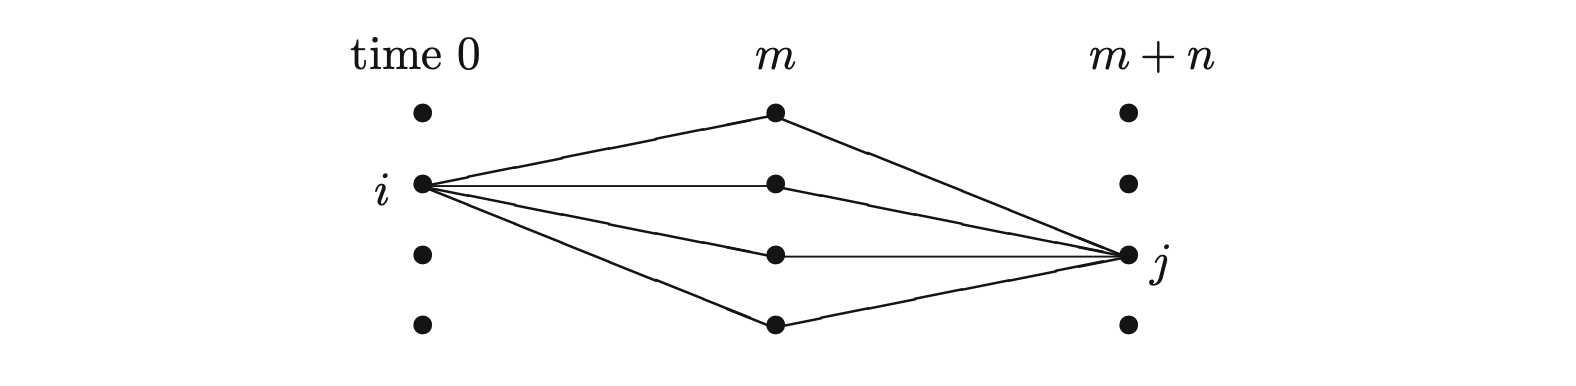
\includegraphics[width=0.9\textwidth]{figures/split_steps.png}
\end{figure}

\newpage